% SI - Figure 1 Flowchart
\begin{figure}[h]
\centering
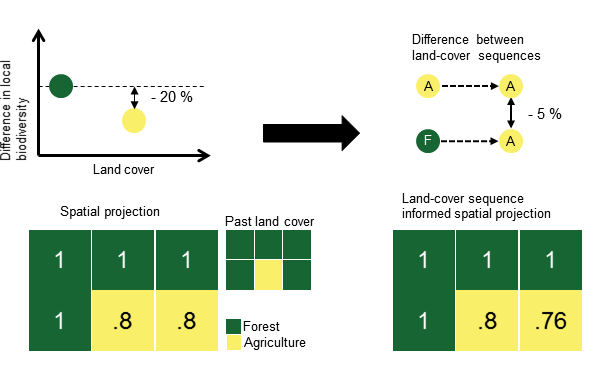
\includegraphics[width=1\textwidth]{chapter2/SI01}
\caption{ Flow chart showing all pre-processing steps of the analysis for both remote sensing and species assemblage data. Remote sensing data were derived from the MODIS Bidirectional reflectance distribution function (BRDF) MCD43A4 product (\href{https://lpdaac.usgs.gov/dataset_discovery/modis/modis_products_table/mcd43a4_v006}{https://lpdaac.usgs.gov/dataset_discovery/modis/modis_products_table/mcd43a4_v006}) and time series of the Enhanced Vegetation Index (EVI) were calculated for the analysis (see Methods). Species assemblage data originates from Projecting Responses of Ecological Diversity In Changing Terrestrial Systems project (PREDICTS, \href{http://www.predicts.org.uk/}{http://www.predicts.org.uk/}). MLE stands for the Maximum Linear Extent as defined by \citep{Hudson2016}.}
\label{SI02_01}
\end{figure}

% SI - Figure 2 Flowchart
\begin{figure}[h]
\centering
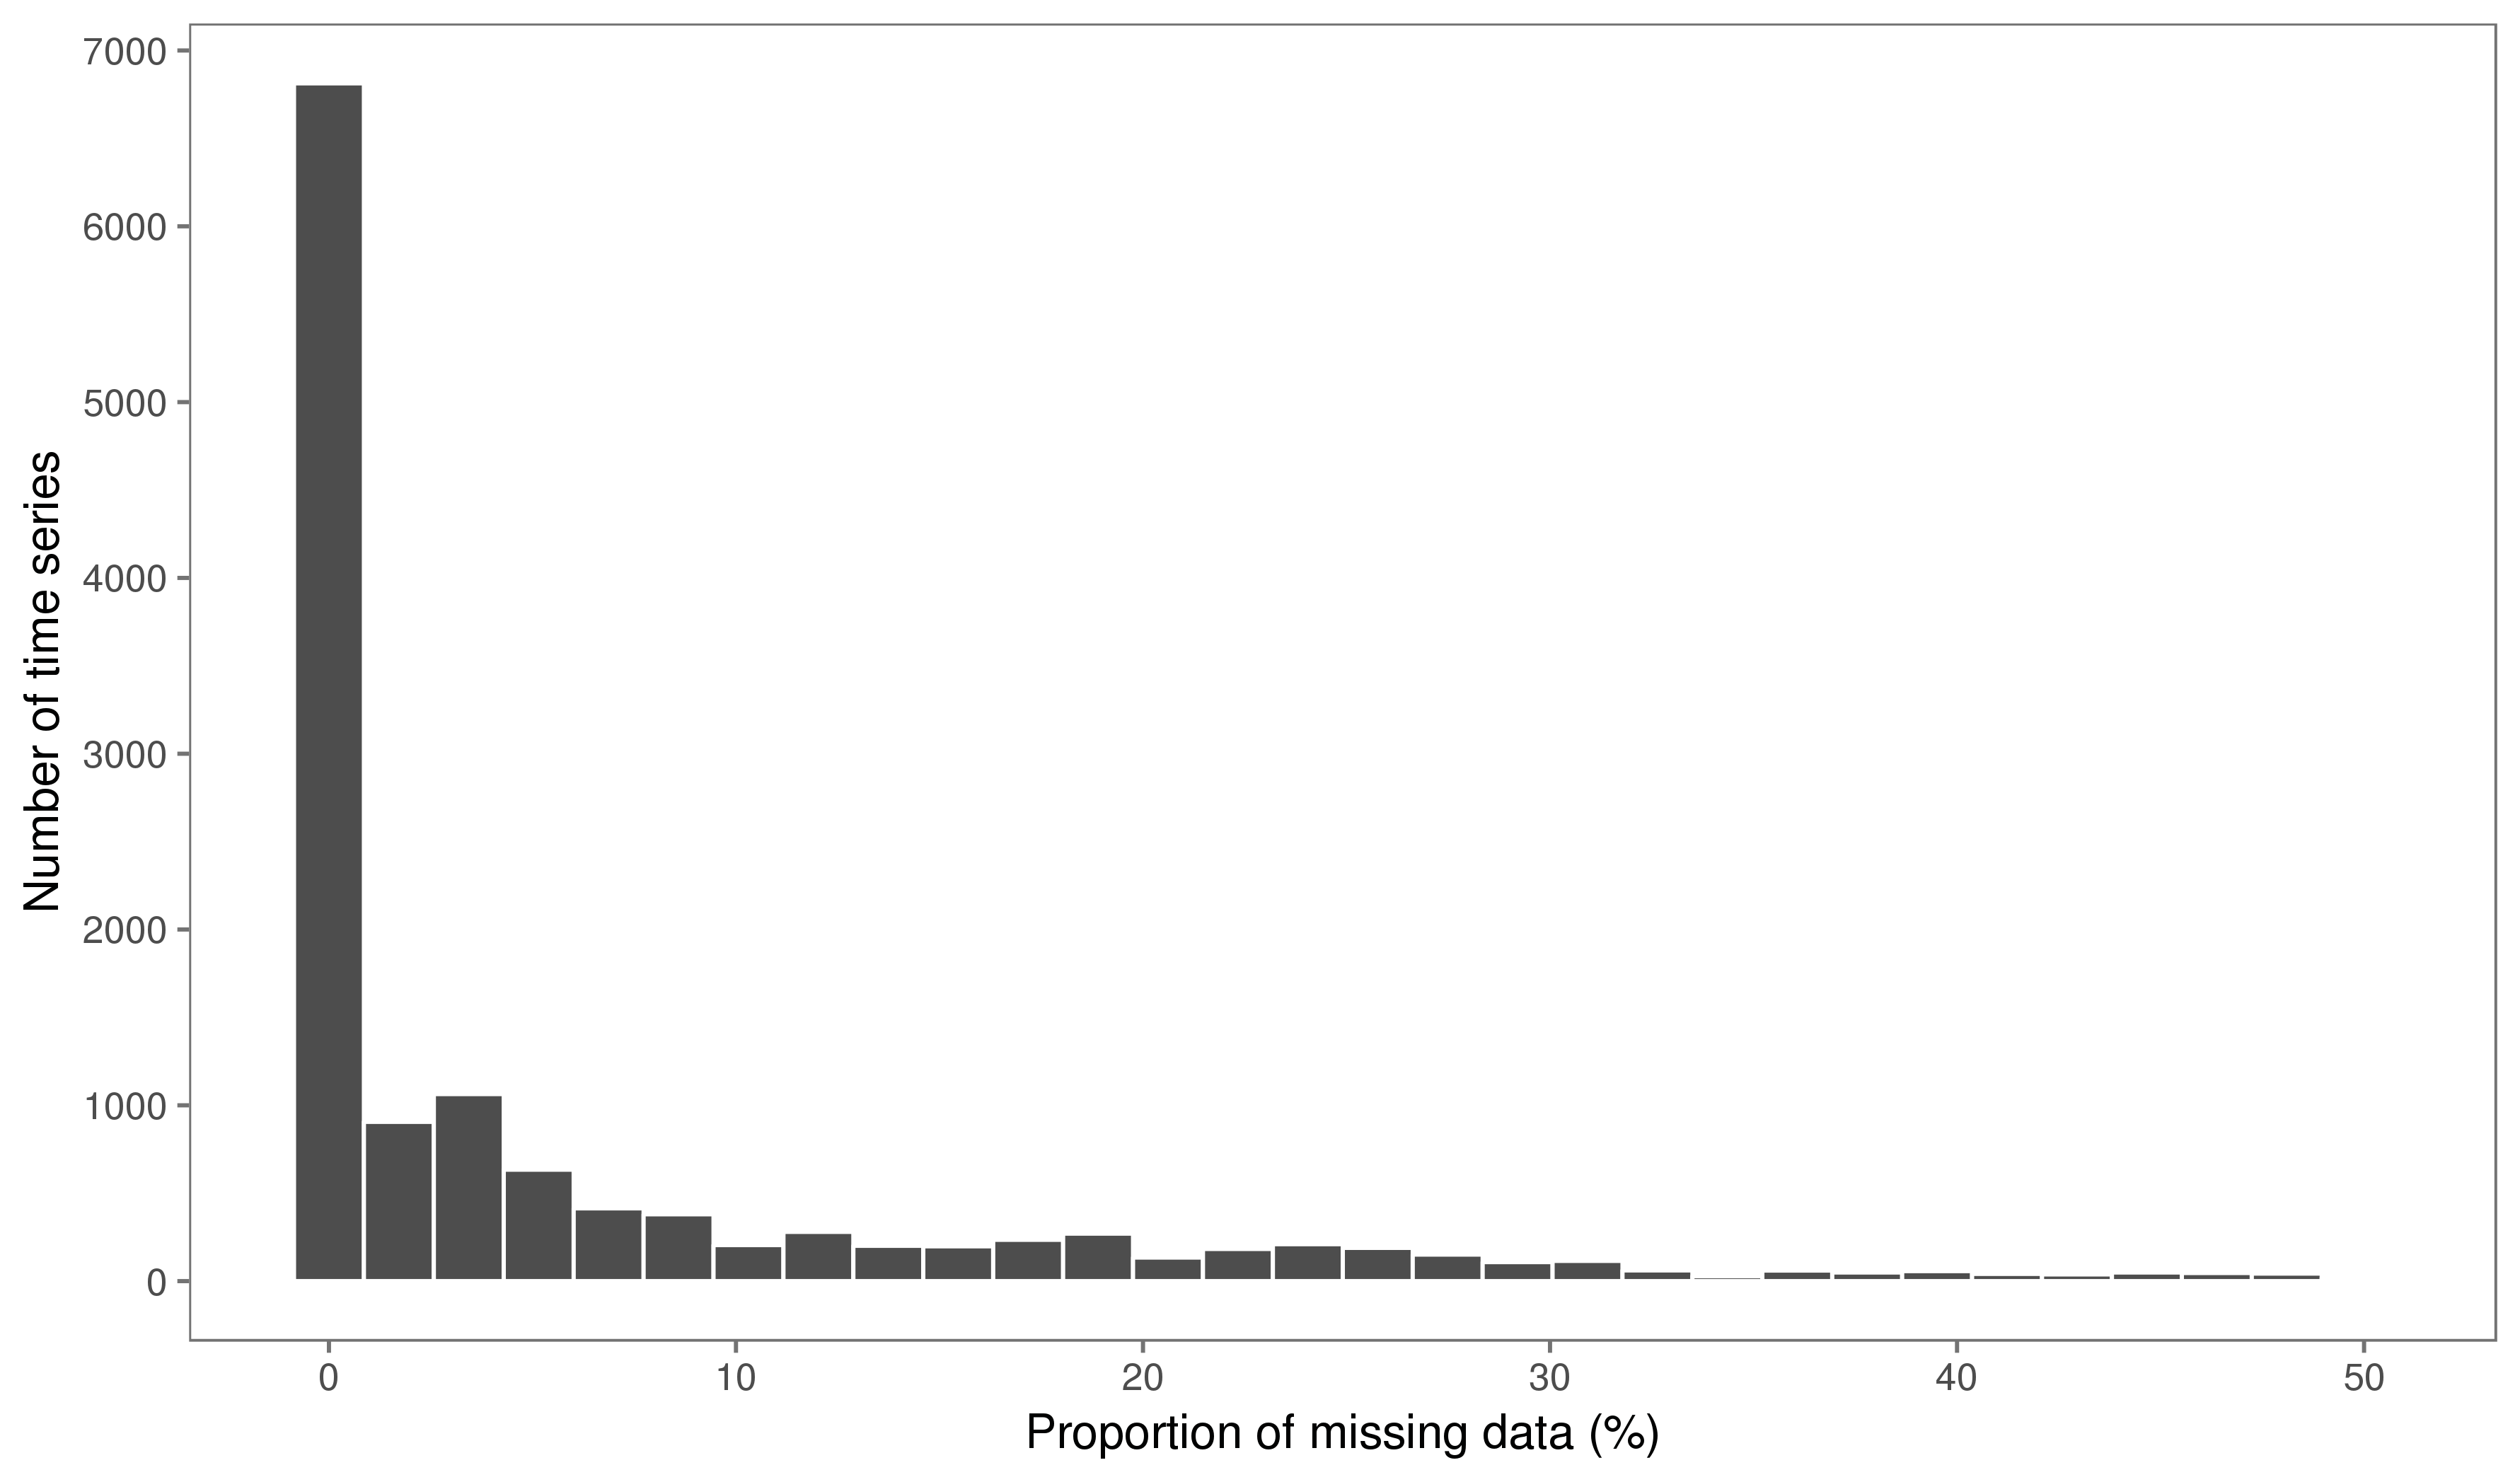
\includegraphics[width=1\textwidth]{chapter2/SI02}
\caption{ Distribution of proportion of missing data (not interpolated) across all time series used. }
\label{SI02_02}
\end{figure}

% SI - Figure 3 Pairwise permutation procedure
\begin{figure}[h]
\centering
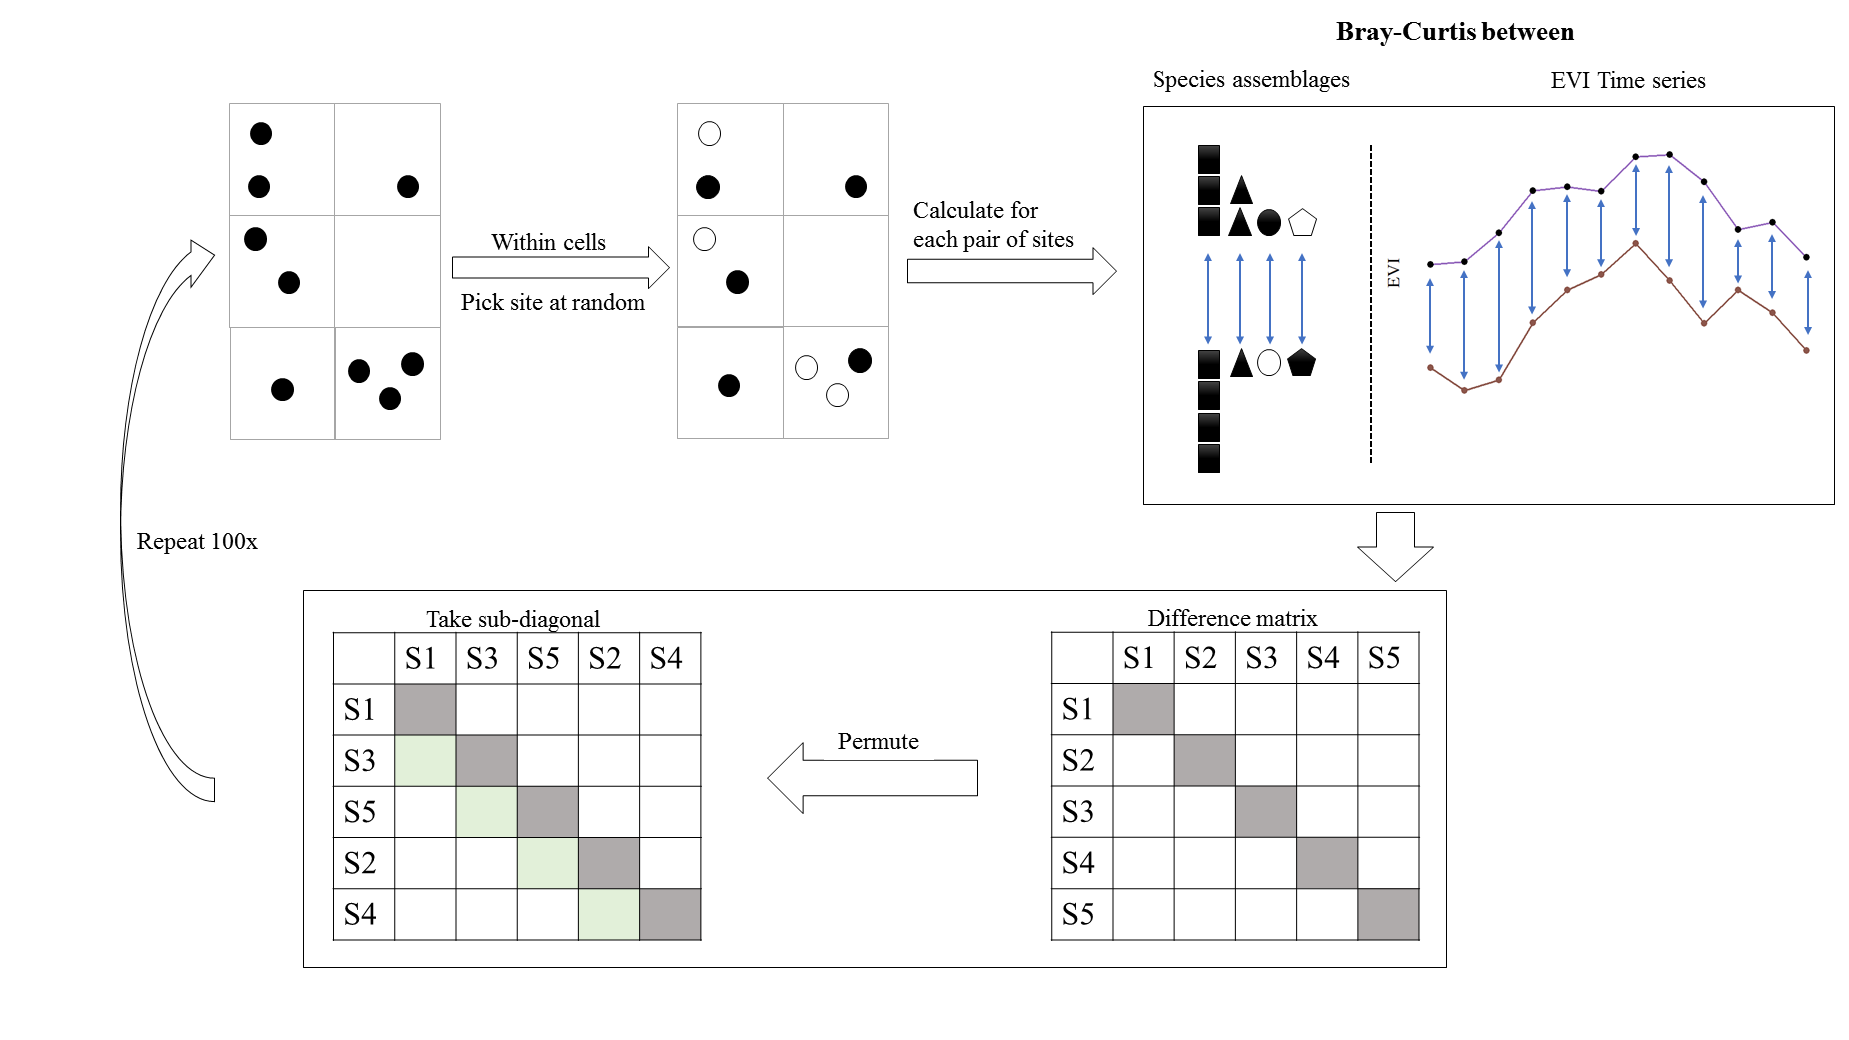
\includegraphics[width=1\textwidth]{chapter2/SI03}
\caption{ Diagram of how the permutations of mutually independent pairwise comparisons were generated. Black dots represent 9 theoretical sites of a study within MODIS grid cells of which one site (S1 – S5) per grid cell was randomly selected. We then calculated two dissimilarity matrices one matrix for the dissimilarity between species assemblages in that grid cell and all other grid cells within the study, and the other matrix for the dissimilarity between time series of the EVI of these grid cells.  For the time series, the Bray-Curtis index was calculated between the EVI values at each time step. For both species assemblages (symbols of varying number and shape) and EVI time series, the obtained dissimilarity matrix was permuted and the sub-diagonal taken for subsequent analysis. }
\label{SI02_03}
\end{figure}

% SI - Figure 4 Pairwise permutation procedure
\begin{figure}[h]
\centering
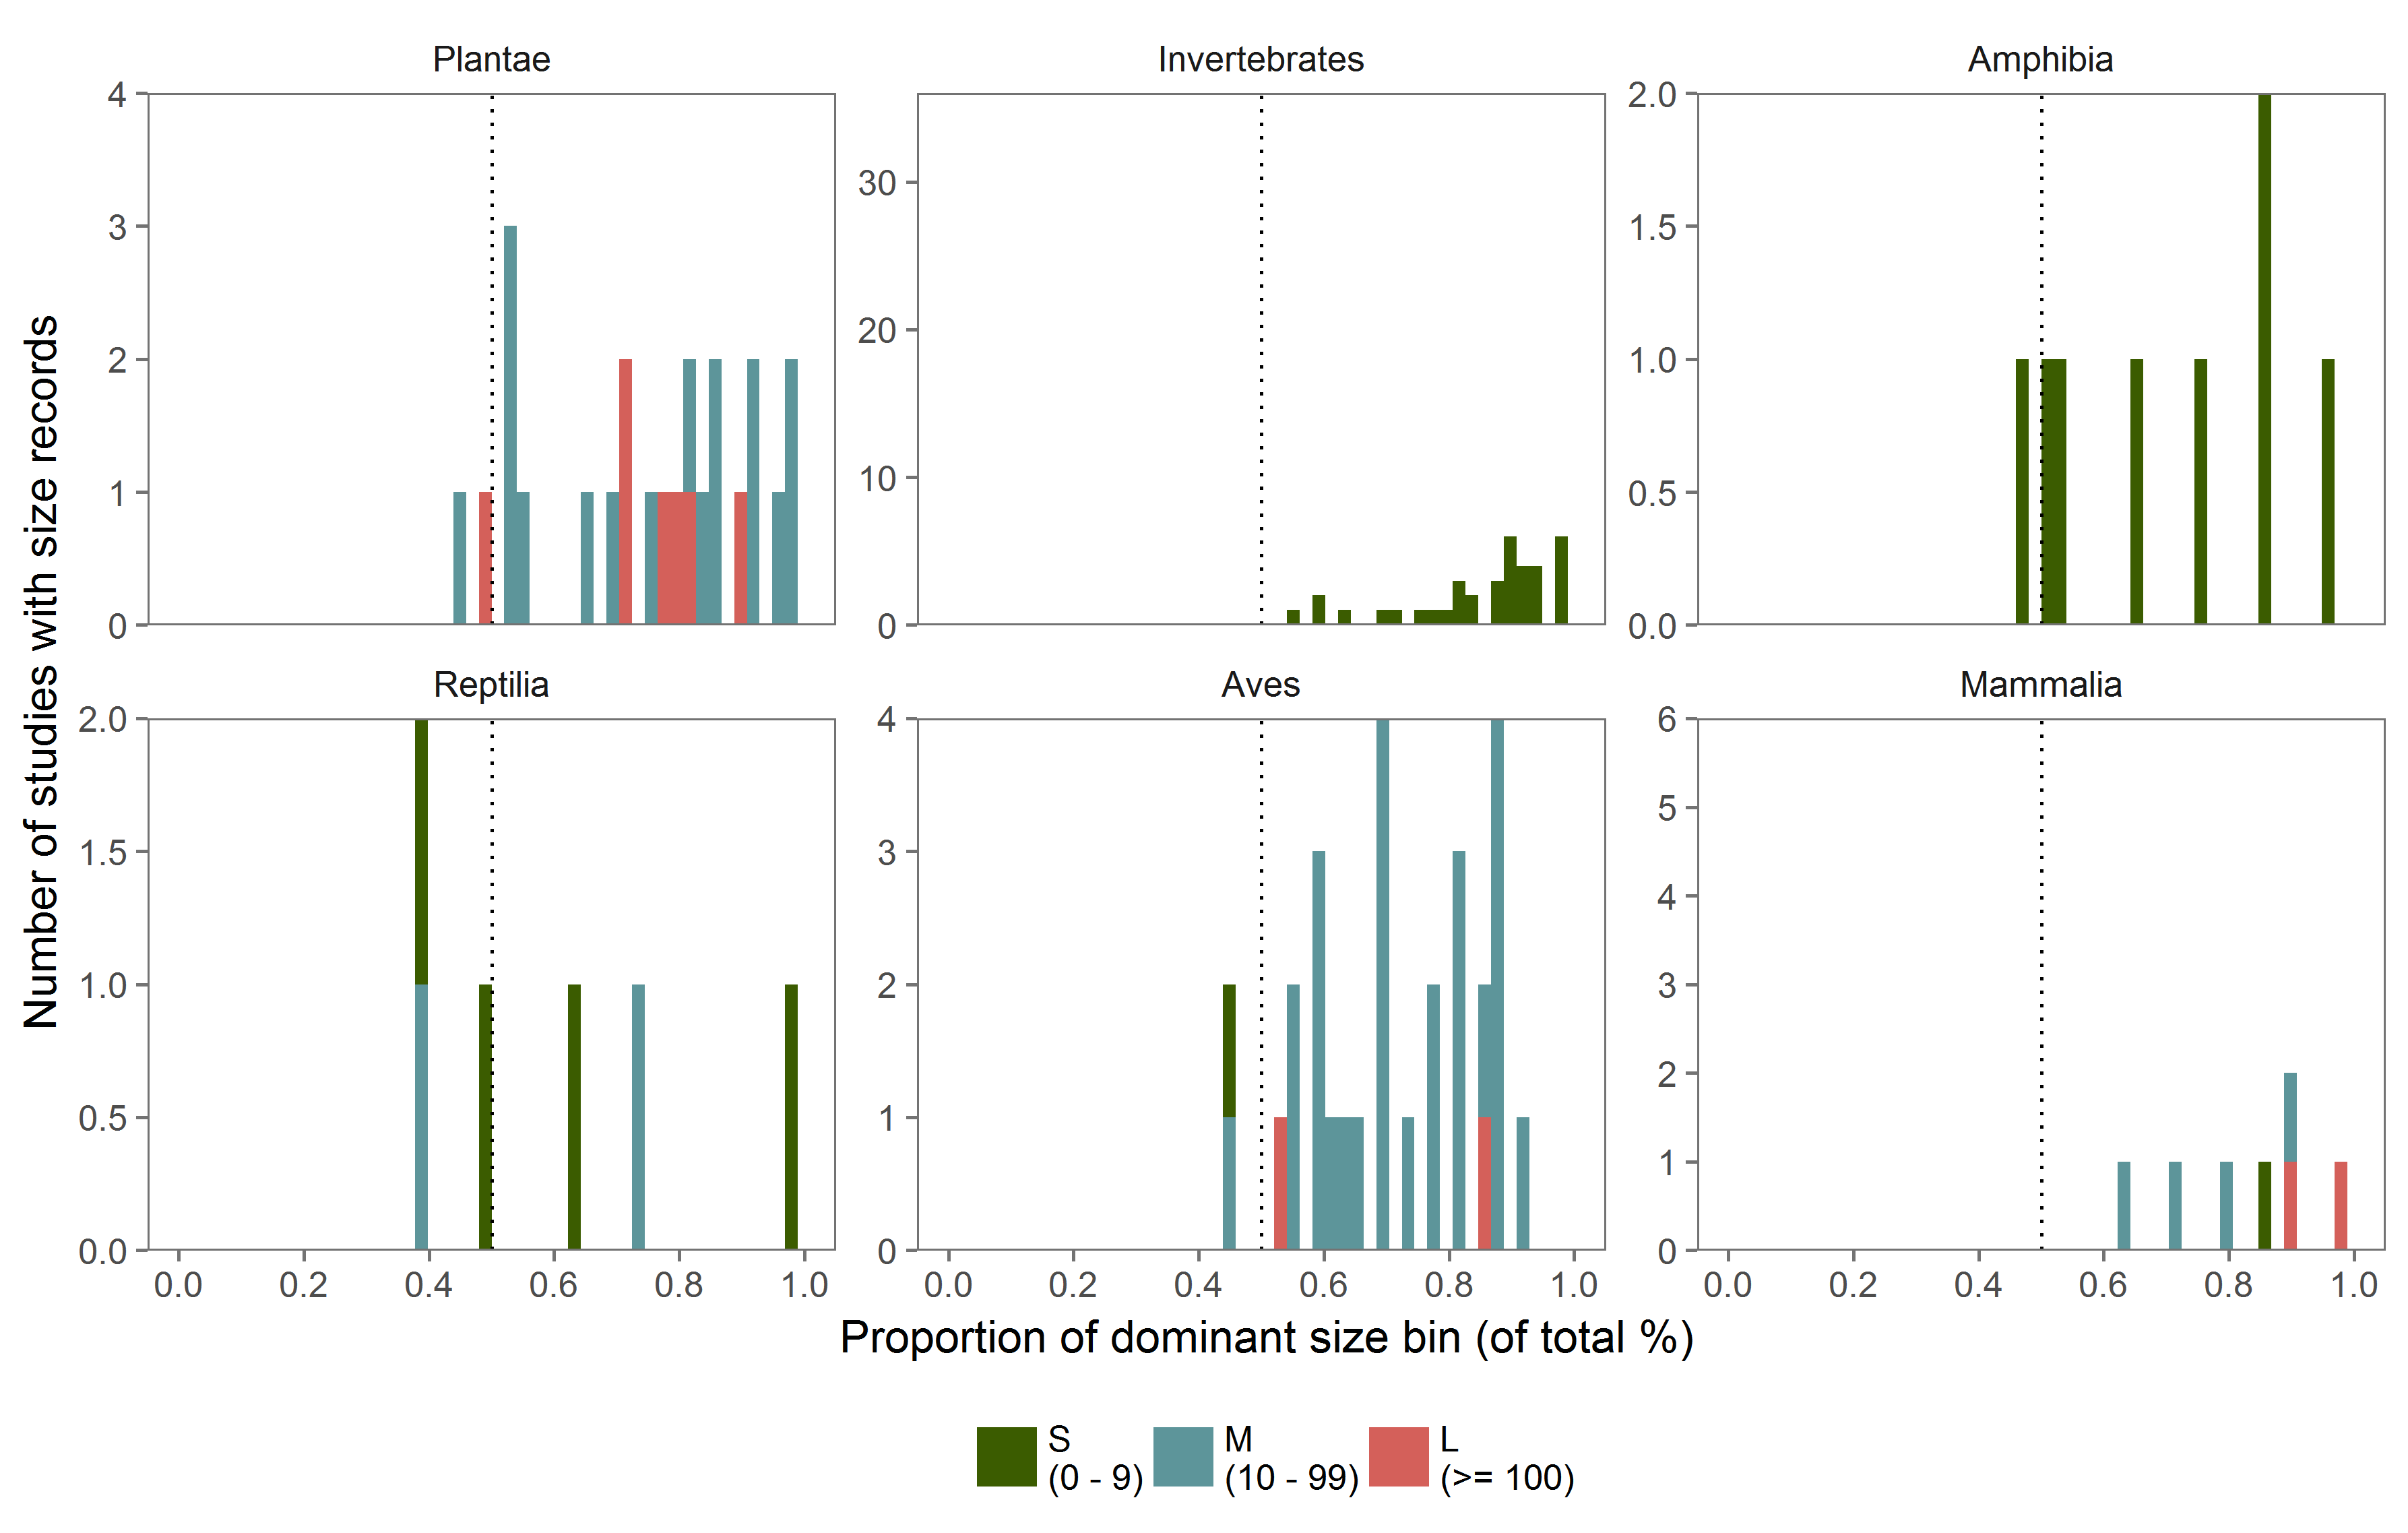
\includegraphics[width=1\textwidth]{chapter2/SI04}
\caption{ The proportion of species that contributed to a study being classified as either predominantly inhabited by small, medium or large species. The dotted line is a visual aid to assess simple majority (50\%) indicating whether a study classification is based on the majority of species within an assemblage. The y-axis shows the number of studies with similar proportions (note the difference in y-axis scale per taxonomic group). }
\label{SI02_04}
\end{figure}
